\documentclass[12pt,letterpaper]{article}
\usepackage[utf8]{inputenc}
\usepackage[spanish, english]{babel}
\usepackage{graphicx}
\usepackage{lettrine}
\usepackage{enumitem}
\usepackage[left=3cm,right=3cm,top=3cm,bottom=3cm]{geometry}
\usepackage{float} 
\usepackage{amsmath}
\usepackage{stackrel} 
\usepackage{multirow}
\usepackage{enumerate}
\renewcommand{\labelitemi}{$-$}
\renewcommand{\labelitemii}{$\cdot$}

\providecommand{\keywords}[1]
{
  \small	
  \textbf{\textit{Keywords: }} #1
}

\providecommand{\pclave}[1]
{
  \small	
  \textbf{\textit{Palabras Clave:}} #1
}
\begin{document}

\title{Caratula}
\begin{titlepage}
\begin{figure}[htb]
\begin{center}

\includegraphics[width=4cm]{./Imagenes/logo.png}
\end{center}
\end{figure}
\vspace*{-0.25in}
\begin{center}
\large{UNIVERSIDAD PRIVADA DE TACNA}\\
\vspace*{-0.025in}
INGENIERIA DE SISTEMAS  \\

\vspace*{0.5in}
\begin{large}
TITULO:\\
\end{large}

\vspace*{0.1in}
\begin{Large}
\textbf{TRABAJO ENCARGADO N° 01} \\
\end{Large}

\vspace*{0.3in}
\begin{Large}
\textbf{CURSO:} \\
\end{Large}

\vspace*{0.1in}
\begin{large}
CALIDAD Y PRUEBAS DE SOFTWARE\\
\end{large}

\vspace*{0.3in}
\begin{Large}
\textbf{DOCENTE:} \\
\end{Large}

\vspace*{0.1in}
\begin{large}
 Ing. Patrick Cuadros Quiroga\\
\end{large}

\vspace*{0.2in}
\vspace*{0.1in}
\begin{large}
Integrantes:\\
\begin{flushleft}
Maldonado Cancapi, Carlos Alejandro\hfill(2018000660) \\
Villanueva Yucra, Josue Joel\hfill(2018000722)\\
Contreras Murguia, Jose Manuel \hfill(2016056346)\\
Rojas Bedregal, Brian Erik\hfill(2018060904)\\
Mamani Laura, Juan Carlos \hfill(2017059565)\\

\end{flushleft}
\end{large}

\vspace*{0.1in}
\begin{large}
Tacna - Perú\\
2021\\

\end{large}
\end{center}

\end{titlepage}

\selectlanguage{spanish}
\begin{abstract}
    Hay una cosa que está clara: por más específico que sea un problema al que se 
    enfrenta durante el desarrollo de su software, existe un 99 por ciento de posibilidades 
    de que alguien haya enfrentado un problema similar en el pasado, que pueda ser modelado de 
    la misma manera.
    Con el modelado queremos decir que la estructura de clases que constituye la solución a su 
    problema puede que ya se haya inventado, porque está resolviendo un problema común que otras 
    personas ya han resuelto antes. Si la forma de resolver este problema se puede extraer, explicar
     y reutilizar en múltiples áreas, entonces nos encontramos ante un patrón de diseño de software.
\end{abstract}
\pclave{estructura de clases, patrón de diseño de software.}

\begin{center}\rule{1\textwidth}{0.05mm} \end{center}

\selectlanguage{english}
\begin{abstract}
    There is one thing that is clear:as specific as it is a problem that you are facing during the development of your software, there is a 99 percent chance that someone has faced such a similar problem in the past, that it can be model in the same way. 
    With modeling we mean that the class structure that makes up the solution to your problem may already have been invented, because you are solving a common problem that other people have already solved before. If the way to solve this problem can be extracted, explained and reused in multiple areas, then we are faced with a software design pattern. 
    
\end{abstract}
\keywords{class structure, software design pattern.}

\selectlanguage{spanish}


\section{Introducción}
A lo largo de la vida de un desarrollador de software se suelen notar diferentes patrones de diseño, en este articulo nos enfocaremos en 
un articulo en específico, el cual tiene como ocupacion la comunicacion entre objetos de clase.
El patron de comportamiento se utiliza para detectar la presencia de patrones de comunicacion ya presentes y pueden manipular dichos patrones.
Estos patrones de diseños estan especificamente relacionados con la comuinicacion entre objetos.
\section{Desarrollo}
\subsection{Patrones de comportamientos}
Se centran en las formas de como interactúan y como se reparten las responsabilidades las distintas clases y objetos.

\subsection{Patrón Observer}
El patrón de diseño Observer permite observar los cambios producidos por un objeto, de esta forma, cada cambio que afecte el estado del objeto observado lanzará una notificación a los observadores; a esto se le conoce como Publicador-Suscriptor. Observer es uno de los principales patrones de diseño utilizados en interfaces gráficas de usuario (GUI), ya que permite desacoplar al componente gráfico de la acción a realizar. 
\subsubsection{Participantes: }
\begin{itemize}

\item IObservable: Interface que deben de implementar todos los objetos que quieren ser observados, en ella se definen los métodos mínimos que se deben implementar. 
\item ConcreteObservable: Clase que desea ser observada, ésta implementa IObservable y debe implementar sus métodos. 
\item IObserver: Interfaces que deben implementar todos los objetos que desean observar los cambios de IObservable. 
\item ConcreteObserver: Clase concreta que está atenta de los cambios de IObserver, esta clase hereda de IObserver y debe de implementar sus métodos.


El patrón de diseño Observer es parecido al patrón Mediator, si bien en él una clase central encapsula y dirige la comunicación generada entre los demás objetos.  


\begin{figure}[h]
\begin{center}
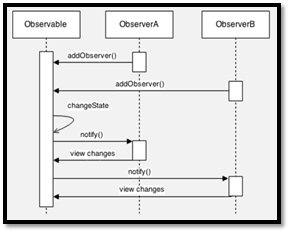
\includegraphics[width=10cm]{./Imagenes/image1.jpg}
\caption{Estructura del patrón de diseño Observer.}
\label{rg1}
\end{center}
\end{figure}
\end{itemize}


\begin{itemize}
\item [1.] El ObserverA se registra con el objeto Observable para ser notificado de algún cambio.
\item [2.] El ObserverB se registra con el objeto Observable para ser notificado de algún cambio. 
\item [3.] Ocurre algún cambio en el estado del Observable. 
\item [4.] Todos los Observers son notificados con el cambio ocurrido. 
    
\end{itemize} 


\subsection{ Patrón Vistor:}
El patrón de diseño Visitor se utiliza para separar la lógica u operaciones que
 se pueden realizar sobre una estructura compleja. En ocasiones nos podemos encontrar 
 con estructuras de datos que requieren realizar operaciones sobre ella, pero estas
  operaciones pueden ser muy variad
  as e incluso se pueden desarrollar nuevas a medida 
  que la aplicación crece. 

\begin{figure}[h]
\begin{center}
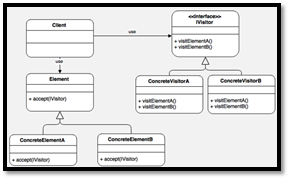
\includegraphics[width=8cm]{./Imagenes/image2.png}
\caption{Estructura del patrón Visitor..}
\label{rg2}
\end{center}
\end{figure}


\subsubsection{Participantes:}
\begin{itemize}
\item Cliente: Componente que interactúa con la estructura (element) y con el Visitante, éste es responsable de crear los visitantes y enviarlos al elemento para su procesamiento. 
\item Element: Representa la raíz de la estructura, en forma de árbol, sobre la que utilizaremos el Visitante. Este objeto por lo general es una interface que define el método accept y deberán implementar todos los objetos de la estructura. 
\item ConcreteElement: Representa un hijo de la estructura compuesta, la estructura completa puede estar compuesta de un gran número de estos objetos y cada uno deberá implementar el método accept. 
\item IVisitor: Interface que define la estructura del visitante, la interface deberá tener un método por cada objeto que se requiera analizar de la estructura (element). 
ConcreteVisitor: Representa una implementación del visitante, esta implementación puede realizar una operación sobre el element. Es posible tener todos los ConcreteVisitor necesarios para realizar las operaciones que necesitemos. 

\end{itemize} 


\begin{figure}[h]
\begin{center}
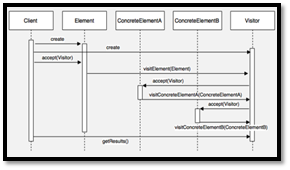
\includegraphics[width=10cm]{./Imagenes/image3.png}
\caption{Diagrama de secuencia del patrón Visitor..}
\label{rg3}
\end{center}
\end{figure}



\begin{itemize}
\item   
\item [1.] El cliente crea la estructura (Element). 
\item [2.] El cliente crea la instancia del Visitante a utilizar sobre la estructura. 
\item [3.] El cliente ejecuta el método accept de la estructura y la envía al Visitante. 
\item [4.] El Element le dice al Visitante con que método lo debe procesar. El Visitante deberá tener un método para cada tipo de clase de la estructura. 
\item [5.] El Visitante analiza al Element mediante su método visitElement y repite el proceso de ejecutar el método accept sobre los hijos del Element. Nuevamente el Visitante deberá tener un método para procesar cada clase hija de la estructura. 
\item [6.] El ConcreteElementA le indica al Visitante con qué método debe procesarlo, el cual es visitElementA. 
\item [7.] La visitante continúa con los demás hijos de Element y esta vez ejecuta el método accept sobre el ConcreteElementB. 
\item [8.] El ConcrteElementB le indica al Visitante con qué método debe procesarlo, el cual es visitElementB. 
\item [9.] Finalmente, el Visitante termina la operación sobre la estructura cuando ha recorrido todos los objetos, obteniendo un resultado que es solicitado por el cliente mediante el método getResults (el resultado es opcional ya que existen operaciones que no arrojan resultados). 
\end{itemize}

\subsection{Patron State: }
El patrón de diseño State se caracteriza por modificar 
su comportamiento dependiendo del estado en el que se encuentra 
la aplicación. Para lograr esto es necesario crear una serie de clases 
que representarán los distintos estados por los que puede pasar la aplicación; es decir, se requiere de una clase por cada estado por el que la aplicación pueda pasar.

\begin{figure}[h]
\begin{center}
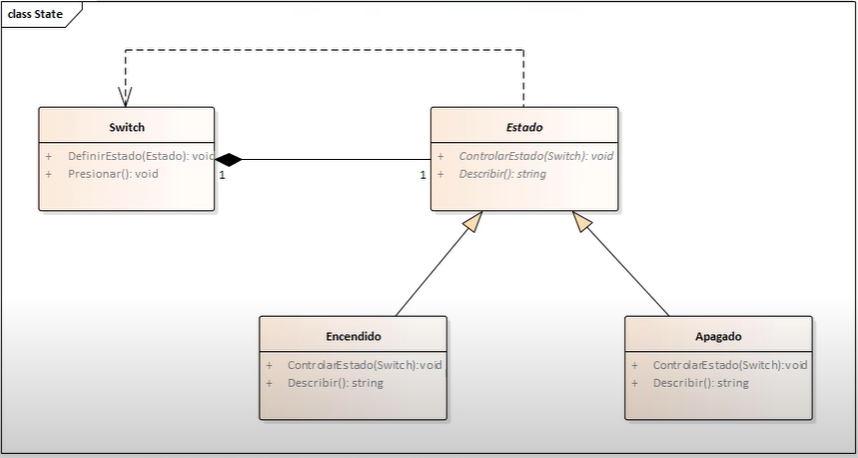
\includegraphics[width=10cm]{./Imagenes/image4.png}
\caption{Estructura del patrón de diseño State.}
\label{rg4}
\end{center}
\end{figure}

\begin{itemize}
    \item Context: Representa el componente que puede cambiar de estado, el cual tiene entre sus propiedades el estado actual. En el ejemplo de la máquina de refrescos, éste sería la máquina como tal.
    \item AbstractState: Clase base para la generación de los distintos estados. Se recomienda que sea una clase abstracta en lugar de una interface debido a que podemos definir comportamientos por default y así afectar el funcionamiento de todos los estados.
    \item ConcreteState: Cada uno de estos componentes representa un posible estado por el cual la aplicación puede pasar, por lo que tendremos un ConcreteState por cada estado posible. Esta clase debe de heredar de AbstractState.
\end{itemize}

\begin{figure}[h]
    \begin{center}
    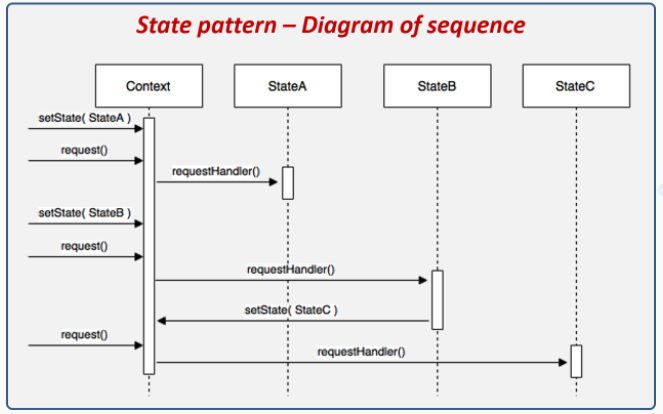
\includegraphics[width=10cm]{./Imagenes/image5.png}
    \caption{Diagrama de secuencia del patrón de diseño State.}
    \label{rg5}
    \end{center}
    \end{figure}
    

\begin{itemize}
    \item [1.] Se establece un estado por default al Context, el cual es StateA.
    \item [2.] Se ejecuta la operación request sobre el Context, la cual delega la ejecución al estado actual (StateA).
    \item [3.] El Context cambia del estado A al estado B.
    \item [4.] Se ejecuta nuevamente la operación request sobre el Context que delega la ejecución al estado actual (StateB).
    \item [5.] La ejecución del StateB da como resultado un cambio de estado al StateC.
    \item [6.] Se ejecuta nuevamente la operación request sobre el Context que delega la ejecución al estado actual (StateC).
\end{itemize}
 


\section{Conclusiones}
    Los patrones de diseño ayudan a estandarizar el código,
    hacen que el diseño sea más comprensible para cuando otros programadores necesiten hacer cambios en el sistema,
    ahora, no se trata de usarlos por usar, tenemos que tener una razon para utilizarlos.
	Los Patrones de diseño son una solución general para problemas conocidos, pero se adaptan de acuerdo a contextos específicos. 
	La mayor complejidad, que representan, es saber cuándo utilizarlos. 

\section{Recomendaciones}
\begin{itemize}
    \item Si no usas patrones, deberías hacerlo. Los patrones ayudan a estandarizar el código, haciendo que el diseño sea más comprensible para otros programadores. Son muy buenas herramientas, y como programadores, siempre deberíamos usar las mejores herramientas a nuestro alcance. 
    \item De nada vale aplicar patrones sin una buena razón. 
    
\end{itemize}
	

\begin{thebibliography}{XXX0000}
\bibitem - Floyd M. (2002). EJB Design Patterns. Canada:Jhon Wiley y Sons, Inc. 
\bibitem - Miguel Angel S. (2017).Patrones de Diseño de Software.Recuperado 7 de Abril 2021, de https://medium.com/all-you-need-is-clean-code/patrones-de-dise%C3%B1o-b7a99b8525e
\bibitem - Gamma E., Helm R., Johnson R., Vlissides J., ; Design Patterns.
Elements of Reusable Object-Oriented Software; AddisonWesley, 1995. Traducción al castellano (2002): Diseño de
patrones. Pearson Educación
\bibitem - Steven J. Metsker, Design Patterns Java Workbook, Addison
Wesley, 2002
\bibitem - Eric Freeman, Elisabeth Freeman, Kathy Sierra, Bert Bates-Head First Design Patterns -OReilly (2008) 
\bibitem - Miriam Martinez Canelo ¿Qué son los patrones de diseño de software?. Recuperado 7 de Abril 2021, de https://profile.es/blog/patrones-de-diseno-de-software/
\bibitem - Oscar Javier Blancarte Iturralde (2016) Introducción a los patrones de diseño: Un enfoque práctico.
\bibitem - Juan Maria Hernandez (2016) Los Patrones de Diseño Hoy: Patrones de Comportamiento. Recuperado 7 de Abril 2021, de https://blog.koalite.com/2016/12/los-patrones-de-diseno-hoy-patrones-de-comportamiento/
\bibitem - Cuizara Porco, Lady Laura. (2019). PATRONES DE DISEÑO DE COMPORTAMIENTO. 
\bibitem - Paloma Díaz, Susana Montero, Ignacio Aedo. (2005). Ingeniería de la web y patrones de diseño.
\end{thebibliography}
\end{document}